\chapter{Incorporating Extra Data into Recommender}
\label{c:incorporating-extra-data}


\newcommand{\norm}[1]{\ensuremath{\lVert{#1}\rVert}}
\newcommand{\Abf}[1]{\ensuremath{\mathbf{#1}}}

In this work we focus in particular on nonlinear methods for collaborative filtering.
After giving an overview of the used notation in the first section, we show a recently developed nonlinear matrix factorization technique as proposed in \cite{Kabbur2015} as part of Section \ref{st:mpcf}.
Section \ref{st:using-extra-data} introduces two models which make use of extra data.
We conclude this chapter with an outline of our software setup in Section \ref{st:system-setup}.

\section{Notation}
\label{st:notation}

As in \cite{Kabbur2015}, all vectors are represented by bold lower case letters, all matrices are represented by bold upper case letters and predicted values are denoted by having a $\hat{}$ (hat) over it.
All important symbols and definitions used in this work is summarized in Table \ref{tab:symbols}.

\begin{table}[p]
	\begin{center}
		\begin{tabularx}{0.9\linewidth}{cX}
			\hline \hline \textbf{Symbol} & \textbf{Definition} \\
			\textit{u, i} & Individual user \textit{u}, item \textit{i} \\
			\textit{n, m} & Number of users and items \\
			\textit{k} & Number of latent factors \\
			\textit{T} & Number of user local preferences \\
			$\mathit{r_{ui}}$ & Rating by user \textit{u} on item \textit{i}\\
			$\mathit{\hat{r}_{ui}}$ & Predicted rating for user \textit{u} on item \textit{i} \\
			\textbf{R} & User-item rating matrix, $\mathbf{R} \in \mathds{R}^{n \times m}$ \\
			\textbf{P} & User latent factor matrix, $\mathbf{P} \in \mathds{R}^{n \times k}$ \\
			\textbf{Q} & Item latent factor matrix, $\mathbf{Q} \in \mathds{R}^{m \times k}$ \\
			\textbf{S} & User latent factor tensor, $\mathbf{S} \in \mathds{R}^{n \times k \times T}$ \\
			$\mathbf{B_u}$ & User-Interest bias matrix, $\mathbf{B_u} \in \mathds{R}^{n \times T}$ \\
			$\mathbf{b_i}$ & Item bias vector, $\mathbf{b_i} \in \mathds{R}^{m}$ \\ 
			$\lambda_{reg}$ & $l_2$-regularization constant\\
			\\
			
			\textit{d} & Number of feature dimensions \\
			$\mathbf{f}_i$ & Feature vector for item \textit{i}, $\mathbf{f}_i \in \mathds{R}^{d}$ \\
			$\mathbf{\hat{f}}_i$ & Predicted feature vector, $\mathbf{\hat{f}}_i \in \mathds{R}^{d}$\\
			\textbf{G} & Weight matrix of the feature prediction model, $\mathbf{G} \in \mathds{R}^{d \times k}$ \\
			\textbf{h} & Bias vector of the feature prediction model, $\mathbf{h} \in \mathds{R}^{d}$ \\
			$\lambda_{ed}$ & Parameter balances matrix factorization model and the feature prediction model \\
			$\lambda_{cos}$ & Parameter balances the Euclidean and the cosine distance \\
			\\
			
			$\mathit{\hat{r}_{ui}^\mathbf{MF}}$ & Predicted rating for user \textit{u} on item \textit{i} of the matrix factorization model \\
			$\hat{e}_{ui}$ & Predicted error\\
			$\mathbf{w}, \mathbf{W^\prime}$ & Weight vector and matrix of the neural network \\
			$\mathbf{x}$ & Input vector to the neural network, $\mathbf{x} \in \mathds{R}^{2k + d}$ \\
			$\varphi(x)$ & Activation function of the neural network \\
			$\lambda_{nn}$ & Parameter balances matrix factorization model and error prediction model \\
			\hline \hline
		\end{tabularx}
	\end{center}
	\caption{Symbols used and definitions}
	\label{tab:symbols}
\end{table}

\section{Nonlinear Matrix Factorization for Collaborative Filtering}
\label{st:mpcf}

\cite{Kabbur2015} developed a nonlinear matrix factorization method called \textbf{MPCF}, which models the user as a combination of global preference and interest-specific latent factors.
In their work, given a user \textit{u}, an item \textit{i} and \textit{T} user local preferences, the estimated rating \textit{$\hat{r}_{ui}$} is given by the sum of the estimations from global preference and interest-specific preference components.
That is,
\begin{equation}
\hat{r}_{ui} = \mu + b_i + \textbf{p}_u \textbf{q}_i^\intercal + \max_{t=1,..,T} (b_{ut} + f(u, i, t)),
\end{equation}
where $\mu$ is the global bias i.e., the average rating value of the entire data set, $b_i$ is the item bias corresponding to item \textit{i}, $b_{ut}$ is the user-local preference bias corresponding to user \textit{u} and local preference \textit{t}, $\textbf{p}_u$ is the latent vector associated with user \textit{u} and $\textbf{q}_i$ is the latent vector associated with item \textit{i} \cite{Kabbur2015}.
\cite{Kabbur2015} proposed two different methods to represent the interest-specific preference component \textit{f(u, i, t)}.
The first one, named \textbf{MPCFi}, has independent item factors in \textit{f(u, i, t)} compared to that of global preference component, whereas the second one shares the item factors of \textit{f(u, i, t)} with the global preference compontent, and thus named \textbf{MPCFs}.
The local preference component \textit{f(u, i, t)} for MPCFs is given by,
\begin{equation}
f(u, i, t) = \textbf{s}_{ut} \textbf{q}_i^\intercal,
\end{equation}
where $\textbf{s}_{ut}$ is the user latent vector for \textit{u} in the local preference component corresponding to the local preference \textit{t} and $\textbf{q}_i^\intercal$ is the shared item latent vector between the global preference and the local preference components \cite{Kabbur2015}.
The following regularized optimization problem is minimized to learn \textbf{P}, \textbf{Q}, \textbf{S}, $\mathbf{B_u}$ and $\mathbf{b_i}$ matrices and vectors:
\begin{equation}
\mathcal{L}_{rating} = \frac{1}{2} \sum_{u,i \in R} (r_{ui} - \hat{r}_{ui})^2 + \frac{\lambda_{reg}}{2} (\norm{\Abf{P}}_F^2 + \norm{\Abf{Q}}_F^2 + \norm{\Abf{S}}_F^2 + \norm{\Abf{B_u}}_F^2 + \norm{\Abf{b_i}}_2^2),\label{eq:mpcf-rating}
\end{equation}
where $r_{ui}$ is the ground truth value,  $\hat{r}_{ui}$ is the estimated value, $\mathbf{b_i}$ is the vector corresponding to the item biases, $\mathbf{B_u}$ is the matrix corresponding to the local preference user biases and $\lambda_{reg}$ is the $l_2$-regularization constant for latent factor matrices \cite{Kabbur2015}.


 

\section{Using Extra Data}
\label{st:using-extra-data}
In this section, we will show how feature vectors were extracted from movie subtitles, then propose two approaches to incorporate such vectors in order to improve top-N recommendations.

\subsection{Feature Extraction from Movie Subtitles}
\label{sst:feature-extraction}
We have downloaded the movie subtitles from a website called Opensubtitles\footnote{Opensubtitles - http://opensubtitles.org}.
Next, a pre-processing step was removing all non-alphanumerical characters which gave us a natural language document per subtitle with an average of 7521 words per document.
With the help of a library called NLTK\footnote{\label{fn:nltk}NLTK - http://www.nltk.org/}, each document was tokenized and stop words were removed.
Gensim\footnote{Gensim - https://radimrehurek.com/gensim/}, a topic modelling library, was then used to generate a feature vector per document via a deep learning algorithm called Paragraph Vectors introduced in \cite{Le2014a}.
The distributed-bag-of-words variant of the Paragraph Vector algorithm and negative sampling was used.
We leave it to \cite{Rong} and \cite{Goldberg2014} in their excellent notes to explain in detail how Word2Vec, the common name of the base algorithm of Paragraph Vectors, works.

\subsection{MPCFs-SI: Regularizing with Extra Data}
\label{sst:mpcfs-si}

\cite{Almahairi2015} have shown that utilizing additional data as a way of regularizing the derived item representations improve the generalization performance of a rating prediction model.
In a similar fashion, we propose to optimize a joint model, which consists of the nonlinear matrix factorization model MPCFs in Eq. \ref{eq:mpcf-rating} and a model which predicts the feature vector of an item $\mathbf{\hat{f}}_i$, given the latent factors for that item $\mathbf{q}_i$.
The feature prediction is modeled as a simple affine transformation of the item latent factors, as shown in Eq.(\ref{eq:affine-transformation}):

\begin{equation}
\hat{\Abf{f}}_{i} = \Abf{G} \Abf{q}_i + \Abf{h} \label{eq:affine-transformation},
\end{equation}
where $\hat{\Abf{f}}_i$ is the predicted feature vector for item $i$, $\Abf{G}$ and $\Abf{h}$ are a weight matrix and a bias vector to be learned.
Since we are transforming from one vector space into another, we have decided to use the squared Euclidean and cosine distances as part of the loss term.
We can informally think of minimizing the Euclidean distance as preserving the magnitude of the vector, while minimizing the cosine distance helps with the vector direction. 
Therefore, the loss term for the feature prediction model is given in Eq. \ref{eq:ed-loss}:
\begin{equation}
\mathcal{L}_{ed} = \sum_{u,i \in R} (\norm{\Abf{f}_i - \hat{\Abf{f}}_i}_F^2 + \lambda_{cos} D_C(\Abf{f}_i, \hat{\Abf{f}}_i)) + \lambda_{reg} \norm{\Abf{G}}_F^2  \label{eq:ed-loss},
\end{equation}
where $\Abf{f}_i$ is a feature vector for item $i$ extracted from movie subtitles via methods discussed in the previous section, $\lambda_{cos}$ is a parameter that balances the performance of the squared Euclidean distance and the cosine distance, $D_C(\Abf{f}_i, \hat{\Abf{f}}_i)$ is the cosine distance and $\lambda_{reg}$ is the $l_2$-regularization constant for the weight matrix.
The cosine similarity $S_C$ and the cosine distance $D_C$ are defined as,

\begin{align}
	S_C(\Abf{a}, \Abf{b}) = \frac{\Abf{a} \cdot \Abf{b}}{\norm{\Abf{a}} \norm{\Abf{b}}} \in [-1, 1] \label{eq:cosine-sim}\\
	D_C(\Abf{a}, \Abf{b}) = 1 - S_C(\Abf{a}, \Abf{b}).
\end{align}
We have also considered modeling the feature prediction with a neural network.
Preliminary results have shown that a neural network model does not improve our metrics.

%\begin{figure}[p]
%	\centering
%	\includegraphics[width=0.5\linewidth]{./section-chapter1/figures/mpcf-si-nn.pdf}
%	\caption[MPCFs-SI: Feature Prediction Model As A Neural Network]
%	{MPCFs-SI: Feature Prediction Model As A Neural Network}
%	\label{f:mpcfs-si-nn}
%\end{figure}

Therefore, the full loss term to optimize is the following:
\begin{equation}
\begin{aligned}
	\mathcal{L} &= \mathcal{L}_{rating} + \lambda_{ed} \mathcal{L}_{ed} \\
				&= \frac{1}{2} \sum_{u,i \in R} (r_{ui} - \hat{r}_{ui})^2 + \frac{\lambda_{reg}}{2} (\norm{\Abf{P}}_F^2 + \norm{\Abf{Q}}_F^2 + \norm{\Abf{S}}_F^2 + \norm{\Abf{B_u}}_F^2 + \norm{\Abf{b_i}}_2^2) \\
				& + \lambda_{ed} (\sum_{u,i \in R} (\norm{\Abf{f}_i - \hat{\Abf{f}}_i}_F^2 + \lambda_{cos} D_C(\Abf{f}_i, \hat{\Abf{f}}_i)) + \lambda_{reg} \norm{\Abf{G}}_F^2),
\end{aligned}
\end{equation}
where $\lambda_{ed}$ is a parameter that balances the performance of the matrix factorization model and the feature prediction model.

We apply AdaGrad, a stochastic gradient descent variant, to update $\mu, \Abf{P}, \Abf{Q}, \Abf{S}, \Abf{B_u}$ and $\Abf{b_i}$.
The gradients for the matrix factorization model are directly from \cite{Kabbur2015}.
We have implemented the feature prediction model in Theano and update $\Abf{G}$ and $\Abf{h}$ with AdaGrad as well.
Theano offers automatic differentiation such that we simply add $\lambda_{ed} \frac{\partial \mathcal{L}_{ed}}{\partial \Abf{q}_i}$ to the item factor gradient $\frac{\partial \mathcal{L}_{rating}}{\partial \Abf{q}_i}$.

As \cite{Kabbur2015} suggest, gradient updates for model parameters are computed for both rated and non-rated entries of $\mathbf{R}$, which is common practice for the top-N recommendation task.
We sample zero entries corresponding to non-rated items on every epoch and add these to the actual training ratings.
\cite{Kabbur2015} indicate that the ratio between rated and non-rated in the range of 1:3 to 1:5 is sufficient to produce the best model.

%The corresponding gradients are as follows:
%
%\begin{equation}
%\begin{aligned}
%-1 \cdot \frac{\partial \mathcal{L}}{\partial b_i} &= (r_{ui} - \hat{r}_{ui}) - \lambda_{reg} b_i \\
%-1 \cdot \frac{\partial \mathcal{L}}{\partial b_{ut^*}} &= (r_{ui} - \hat{r}_{ui}) - \lambda_{reg} b_{ut^*} \\
%-1 \cdot \frac{\partial \mathcal{L}}{\partial \Abf{p}_u} &= (r_{ui} - \hat{r}_{ui}) \Abf{q}_i - \lambda_{reg} \Abf{p}_u \\
%-1 \cdot \frac{\partial \mathcal{L}}{\partial \Abf{q}_i} &= (r_{ui} - \hat{r}_{ui}) (\Abf{p}_u + \Abf{w_{ut^*}}) + \lambda_{ed} ((\Abf{f}_i - \hat{\Abf{f}}_i) \cdot \Abf{G})^\intercal - \lambda_{reg} \Abf{q}_i \\
%-1 \cdot \frac{\partial \mathcal{L}}{\partial \Abf{s}_{ut^*}} &= (r_{ui} - \hat{r}_{ui}) \Abf{q}_i - \lambda_{reg} \Abf{s}_{ut^*} \\
%-1 \cdot \frac{\partial \mathcal{L}}{\partial \Abf{G}} &= \lambda_{ed} (\Abf{f}_i - \hat{\Abf{f}}_i) \cdot \Abf{q}_i - \lambda_{reg} \Abf{G} \\
%-1 \cdot \frac{\partial \mathcal{L}}{\partial \Abf{h}} &= \lambda_{ed} (\Abf{f}_i - \hat{\Abf{f}}_i)
%\end{aligned}
%\end{equation}
%where $t^*$ is the local preference corresponding to maximum score of the local preference component.

When we use the introduced feature prediction model together with the nonlinear matrix factorization model MPCFs, we call this joint model \textbf{MPCFs-SI}.

\subsection{MFNN: Neural Network}
\label{sst:mfnn}

The second model we propose is an ensemble of a matrix factorization model and a neural network model.
We call this joint model \textbf{MFNN}.
It is inspired by the MPCFs model and has the benefit of being able to directly incorporate additional user or item data as input to the neural network.

The estimated rating \textit{$\hat{r}_{ui}$} is given by:

\begin{align}
	\hat{r}_{ui} &= \hat{r}_{ui}^\mathbf{MF} + \hat{e}_{ui},\\
	\hat{r}_{ui}^\mathbf{MF} &= \mu + b_i + \textbf{p}_u \textbf{q}_i^\intercal,
\end{align}
where $\hat{r}_{ui}^\mathbf{MF}$ is the predicted rating of the matrix factorization model, and $\hat{e}_{ui}$ is the predicted error modeled in a neural network.
The actual error and the predicted error are defined as,
\begin{align}
	e_{ui} &= r_{ui} - \hat{r}_{ui}^\mathbf{MF}, \\
	\hat{e}_{ui} &= \sum_j (w_{j} \varphi(\sum_l^{} w^\prime_{j,l} x_l)),\\
	\mathbf{x} &= (\mathbf{p}_u, \mathbf{q}_i, \mathbf{f}_i), \\
	\varphi(x) &= max(0, x),
\end{align}
where $w_{\cdot}$ and $w_{\cdot,\cdot}^\prime$ are weights of the neural network model to be learned, $\mathbf{x}$ is a concatenation of the user latent factors $\mathbf{p}_u$, the item latent factors $\mathbf{q}_i$ and the side information as a feature vector $\mathbf{f}_i$, $j$ is the number of neurons in the hidden layer, $l$ is the length of $\mathbf{x}$ and $\varphi(x)$ is the activation function.
Figure \ref{f:mfnn} shows the neural network in a diagram.

The loss term for this joint model is as follows:
\begin{equation}
\begin{aligned}
\mathcal{L} &= \frac{1}{2} \sum_{u,i \in R} (r_{ui} - \hat{r}_{ui}^\mathbf{MF})^2 + \frac{\lambda_{reg}}{2} (\norm{\Abf{P}}_F^2 + \norm{\Abf{Q}}_F^2 + \norm{\Abf{b_i}}_2^2) \\
& + \frac{\lambda_{nn}}{2} (\sum_{u,i \in R} (e_{ui} - \hat{e}_{ui})^2 + \lambda_{reg} (\norm{\Abf{w}}_F^2 + \norm{\Abf{W^\prime}}_F^2)),
\end{aligned}
\end{equation}
where $\lambda_{nn}$ is a parameter that balances the performance of the matrix factorization model and the error prediction of the neural network model.

As in the previous model MPCFs-SI, we apply AdaGrad to update $\mu, \Abf{P}, \Abf{Q},$ and $\Abf{b_i}$.
The neural network model is implemented in Theano and its parameters get updated via AdaGrad.
The sampling of non-rated items is done the same way as in our first model.

\begin{figure}[p]
	\centering
	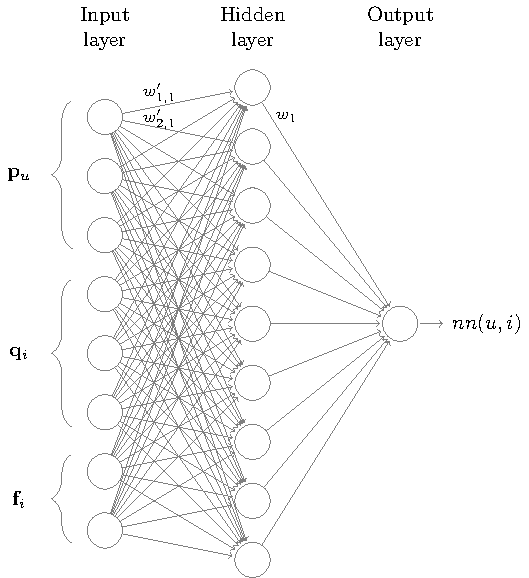
\includegraphics[width=0.9\linewidth]{./section-chapter1/figures/mfnn.pdf}
	\caption[MFNN: Neural Network]
	{MFNN: Neural Network}
	\label{f:mfnn}
\end{figure}

\section{System Setup}
\label{st:system-setup} 

We have built a custom software in Python.
The two models just introduced as well as the baseline recommender MPCFs \cite{Kabbur2015} and \textbf{BPRMF} \cite{Rendle2009} were implemented by us.
For the baseline recommender \textbf{SLIM} \cite{Ning2011}, we were able use parts of an open source implementation by Mendeley\footnote{Mendeley mrec - https://github.com/Mendeley/mrec}.
Data handling was done with the Pandas library and we have used Numpy for linear algebra operations.
As explained in Section \ref{sst:feature-extraction}, feature vectors for the movies were extracted from their subtitles with the help of Gensim\footnote{Gensim - https://radimrehurek.com/gensim/} and NLTK\footnote{NLTK - http://www.nltk.org/}.
All neural network related functionalities were implemented with Lasagne\footnote{Lasagne - https://github.com/Lasagne/Lasagne} and Theano\footnote{Theano - http://deeplearning.net/software/theano/}.
The source code for this work can be downloaded under https://github.com/marcuniq/bsc-thesis.
